\documentclass{article}
\usepackage[utf8]{inputenc}
\usepackage{graphicx}
\usepackage{hyperref}
\title{Introduction To Research}
\author{Omolade Ikumapayi}
\date{August 2022}

\begin{document}

\maketitle

\section{Introduction}

\begin{figure}[h!]
  \centering
  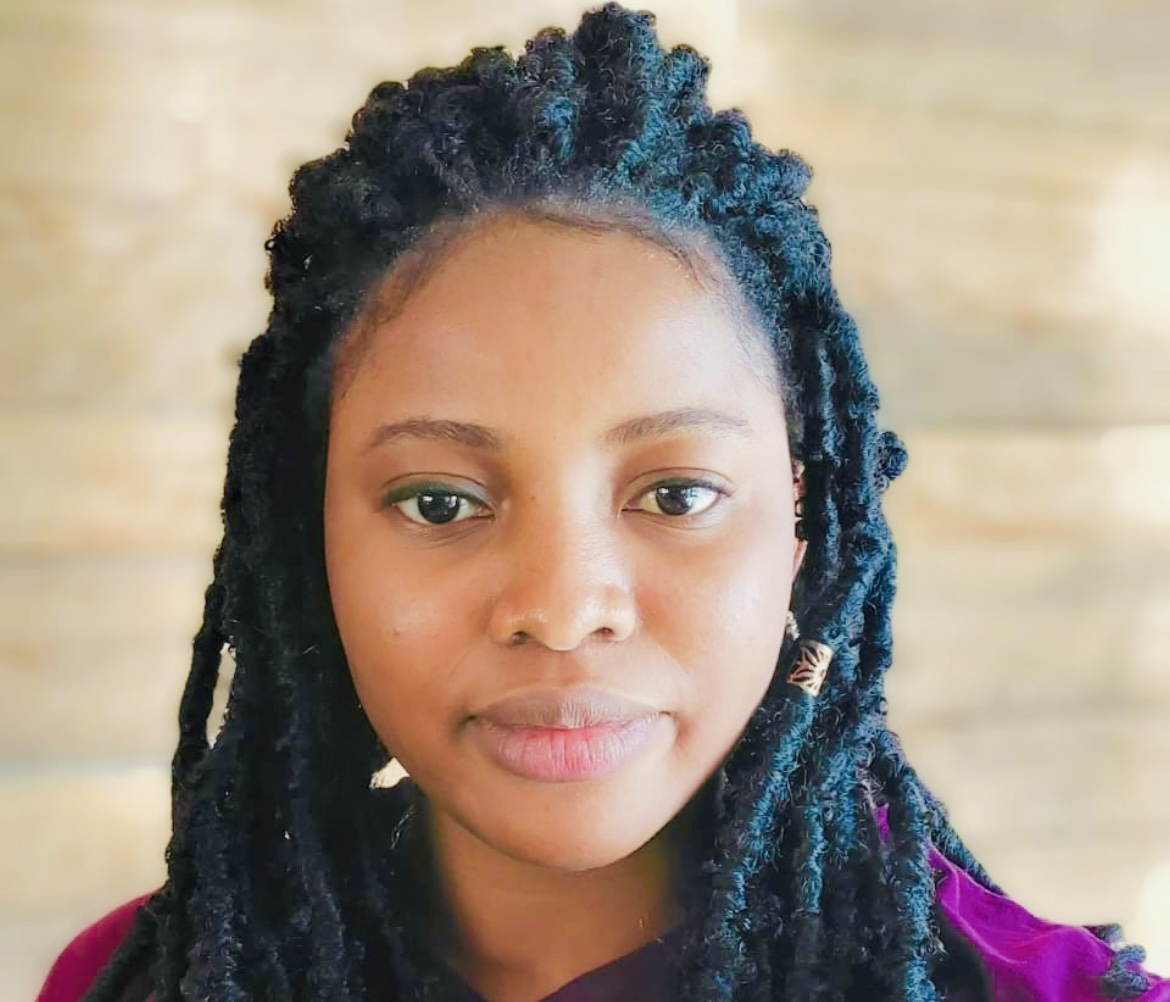
\includegraphics[width=0.5\textwidth]{omolade_.jpg}
\end{figure}

I am a second-year Ph.D. student in the department of computer science at the University of Colorado, Colorado Springs. I work with Dr.Gedare Bloom at the Embedded System Security Laboratory on real-time systems security. Currently I am investigating scheduling algorithms for automotive applications. My goal for taking Introduction to Research class is to get better at research. I believe research is a process and I want to go through the cycle. I consider myself to be creative as I enjoy designing, yet it can be difficult to put ideas into words, and have a thorough statistical and technical representation through the examination of my ideas.
I hope to explore and understand sophisticated scientific publications through this course, which will assist me to get past my research challenges. As someone who wants to increase the caliber of her research, I am also taking this course to network with others who share my interests.
Finally, I believe that by the end of the class, I will have gained the necessary knowledge, skills, and experience to  maximize my potential. With in-depth research, I hope to improve my understanding of the nuances of Cyber-physical systems and take advantage of the opportunity to be taught by the course coordinator. I intend to contribute to the field by applying my theoretical knowledge and scientific ingenuity.
\section{Git Repository}

\url{https://gitlab.com/ipvs/nesting}
\section{Questions}
\subsection{Question 1}
Hi Omolade. Your goal is spot on! Do you intend to do more research or more teaching after the program or maybe a combination of both? Thanks ..Rono

\subsection{Question 2}
\end{document}
